\chapter{Modeling the Earth with Fatiando a Terra}
\label{chap:fatiando}


This chapter was published in the Proceedings of the 12th Python in Science
Conference in 2013
(\url{http://conference.scipy.org/proceedings/scipy2013/uieda.html}).
It describes the open-source software library Fatiando a Terra and the state of
the project at the time of the conference.
Fatiando a Terra was developed by me as part of my PhD thesis work.
The library has grown since 2013 and now contains more features than described
here.
For example, the algorithm for gravitational forward modeling with tesseroids
presented in Chapter~\ref{chap:tesseroids} is also implemented in Fatiando a
Terra.
Furthermore, the gravity inversion method presented in Chapter~\ref{chap:moho}
is implemented using functions and classes from Fatiando a Terra and will be
included in a future release of the library.
The official website (\url{http://www.fatiando.org}) contains more up-to-date
information about the project.



\section{Abstract}

Geophysics is the science of using physical observations of the Earth to infer
its inner structure. Generally, this is done with a variety of numerical
modeling techniques and inverse problems. The development of new algorithms
usually involves copy and pasting of code, which leads to errors and poor code
reuse. Fatiando a Terra is a Python library that aims to automate common tasks
and unify the modeling pipeline inside of the Python language. This allows
users to replace the traditional shell scripting with more versatile and
powerful Python scripting. The library can also be used as an API (Application
Programming Interface) for developing stand-alone programs.  Algorithms
implemented in Fatiando a Terra can be combined to build upon existing
functionality. This flexibility facilitates prototyping of new algorithms and
quickly building interactive teaching exercises. In the future, we plan to
continuously implement sample problems to help teach geophysics as well as
classic and state-of-the-art algorithms.




\section{Introduction}

Geophysics studies the physical processes of the Earth. Geophysicists make
observations of physical phenomena and use them to infer the inner structure of
the planet. This task requires the numerical modeling of physical processes.
These numerical models can then be used in inverse problems to infer inner
Earth structure from observations. Different geophysical methods use different
kinds of observations. Geothermal methods use the temperature and heat flux of
the Earth's crust.  Potential field methods use gravitational and magnetic
field measurements. Seismics and seismology use the ground motion caused by
elastic waves from active (man-made) and passive (earthquakes) sources,
respectively.

The seismic method is among the most widely studied due to the high industry
demand. Thus, a range of well established open-source software have been
developed for seismic processing. These include Seismic Un*x \citep[][
\url{http://www.cwp.mines.edu/cwpcodes/}]{stockwelljr.1999}, Madagascar
\citep[][ \url{http://www.ahay.org/}]{madagascardevelopmentteam2013}, OpendTect
(\url{http://opendtect.org}), and GêBR (\url{http://www.gebrproject.com}). A
noteworthy open-source project that is not seismic related is the Generic
Mapping Tools (GMT) project \citep[][
\url{http://gmt.soest.hawaii.edu/}]{wessel1991}. The GMT are a well established
collection of command-line programs for plotting maps with a variety of
different map projections.  For geodynamic modeling there is the Computational
Infrastructure for Geodynamics (\url{http://www.geodynamics.org}), which has
grouped various well documented software packages. However, even with this wide
range of well maintained software projects, many geophysical modeling software
that are provided online still have no open-source license statement, have
cryptic I/O files, are hard to integrate into a pipeline, and make code reuse
and remixing challenging. Some of these problems are being worked on by the
Solid Earth Teaching and Research Environment (SEATREE) \citep[][
\url{http://geosys.usc.edu/projects/seatree/}]{milner2009} by providing a
common graphical interface for previously existing software. The numerical
computations are performed by the pre-existing underlying C/Fortran programs.
Conversely, the SEATREE code (written in Python) handles the I/O and user
interface. This makes the use of these tools easier and more approachable to
students. However, the lack of a common Application Programming Interface (API)
means that the code for these programs cannot be easily combined to create new
modeling tools.

Fatiando a Terra (\url{http://www.fatiando.org}) aims at providing such an API
for geophysical modeling. Functions in the \texttt{fatiando} package use
compatible data and mesh formats so that the output of one modeling function
can be used as input for another. Furthermore, routines can be combined and
reused to create new modeling algorithms.  Fatiando a Terra also automates
common tasks such as griding, map plotting with Matplotlib \citep[][
\url{http://matplotlib.org}]{hunter2007}, and 3D plotting with Mayavi \citep[][
\url{http://code.enthought.com/projects/mayavi}]{ramachandran2011}.  Version
0.1\footnote{
    This was the current version in 2013 when this chapter was published in the
    conference proceedings. As of April 2016, the latest version is 0.3.}
of Fatiando a Terra is focused on gravity and magnetic methods because this is
the main focus of the developers.  However, simple ``toy'' problems for
seismology and geothermics are available and can be useful for teaching
geophysics.

The following sections illustrate the functionality and design of Fatiando a
Terra using various code samples. An IPython \citep[][
\url{http://ipython.org/}]{perez2007} notebook file with these code samples is
provided by \citet{uieda2013} at
\url{http://dx.doi.org/10.6084/m9.figshare.708390}.



\section{Package structure}

The modules and packages of Fatiando a Terra are bundled into the
\texttt{fatiando} package. Each type of geophysical method has its own
package. As of version 0.1, the available modules and packages are:

\begin{itemize}
\item
  \texttt{fatiando.gravmag}: gravity and magnetic methods;
\item
  \texttt{fatiando.seismic}: seismic methods and seismology;
\item
  \texttt{fatiando.geothermal}: geothermal modeling;
\item
  \texttt{fatiando.mesher}: geometric elements and meshes;
\item
  \texttt{fatiando.gridder}: grid generation, slicing, interpolation,
  etc;
\item
  \texttt{fatiando.io}: I/O of models and data sets from web
  repositories;
\item
  \texttt{fatiando.utils}: miscellaneous utilities;
\item
  \texttt{fatiando.constants}: physical constants;
\item
  \texttt{fatiando.gui}: simple graphical user interfaces;
\item
  \texttt{fatiando.vis}: 2D and 3D plotting;
\item
  \texttt{fatiando.inversion}: inverse problem solvers and
  regularization;
\end{itemize}

\section{Griding and map plotting}

Fatiando a Terra handles map data as 1D Numpy arrays, typically x-, y-,
z-coordinates and an extra array with the corresponding data. However,
Matplotlib functions, like \texttt{contourf} and \texttt{pcolor},
require data to be passed as 2D arrays. Moreover, geophysical data sets
are often irregularly sampled and require griding before they can be
plotted. Thus, griding and array reshaping are ideal targets for
automation.

The \texttt{fatiando.vis.mpl} module imports all the functions in
\texttt{matplotlib.pyplot}, adds new functions, and overwrites others to
automate repetitive tasks (such as griding). Thus, the basic
functionality of the \texttt{pyplot} interface is maintained while
customizations facilitate common tasks. The following example
illustrates the use of the custom \texttt{fatiando.vis.mpl.contourf}
function to automatically grid and plot some irregularly sampled data
(Figure~\ref{fig:p1-contourf}):

\begin{verbatim}
from fatiando import gridder
from fatiando.vis import mpl
area = [-20, 20, -50, 50]
x, y = gridder.scatter(area, n=100)
data = x**2 + y**2
mpl.figure()
mpl.axis('scaled')
mpl.contourf(y, x, data, shape=(50, 50),
    levels=30, interp=True)
mpl.colorbar(orientation='horizontal')
mpl.plot(y, x, '.k')
mpl.xlabel('y (East-West)')
mpl.ylabel('x (North-South)')
mpl.show()
\end{verbatim}


\begin{figure}
    \centering
    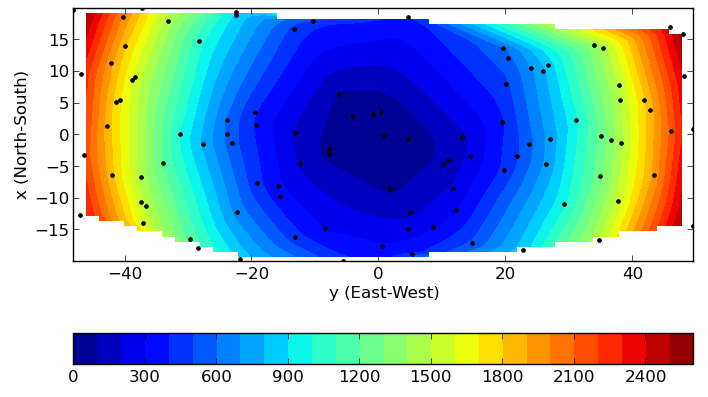
\includegraphics[width=\textwidth]{figures/paper-fatiando/gridding_plotting_contourf}
    \caption{
    Example of 1) generating a random scatter of points (black dots),
    2) using that to make synthetic data, and
    3) automatically gridding and plotting the data using a
    Fatiando a Terra wrapper for the Matplotlib ``contourf``
    function.
    }
    \label{fig:p1-contourf}
\end{figure}


Notice that, in the calls to \texttt{mpl.contourf} and
\texttt{mpl.plot}, the x- and y-axis are switched. That is because it is
common practice in geophysics for x to point North and y to point East.

Map projections in Matplotlib are handled by the
Basemap toolkit (\url{http://matplotlib.org/basemap}). The
\texttt{fatiando.vis.mpl} module also provides helper functions to
automate the use of this toolkit. The \texttt{fatiando.vis.mpl.basemap}
function automates the creation of the \texttt{Basemap} objects with
common parameters. This object can then be passed to the
\texttt{contourf}, \texttt{contour} and \texttt{pcolor} functions in
\texttt{fatiando.vis.mpl} and they will automatically plot using the
given projection (Figure~\ref{fig:p1-basemap}):

\begin{verbatim}
mpl.figure()
bm = mpl.basemap(area, projection='robin')
bm.drawmapboundary()
bm.drawcoastlines()
mpl.contourf(x, y, data, shape=(50, 50), levels=30,
    interp=True, basemap=bm)
mpl.colorbar(orientation='horizontal')
mpl.show()
\end{verbatim}

\begin{figure}
    \centering
    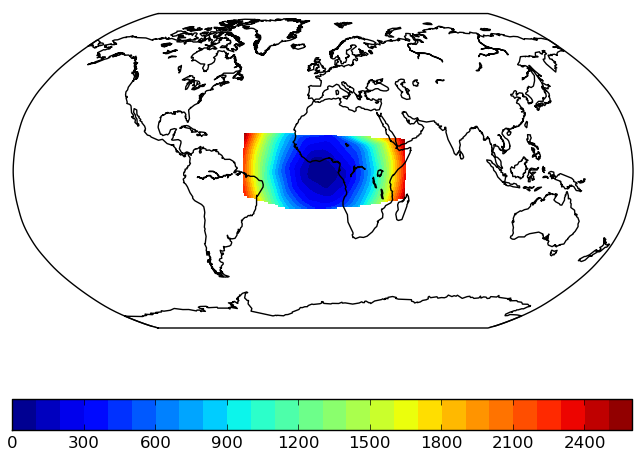
\includegraphics[width=\textwidth]{figures/paper-fatiando/gridding_plotting_basemap}
    \caption{
        Example of map plotting with the Robinson projection using the
        Matplotlib Basemap toolkit.
    }
    \label{fig:p1-basemap}
\end{figure}



\section{Meshes and 3D plotting}

The representation of 2D and 3D geometric elements is handled by the
classes in the \texttt{fatiando.mesher} module. Geometric elements in
Fatiando a Terra can be assigned physical property values, like density,
magnetization, seismic wave velocity, impedance, etc. This is done
through a \texttt{props} dictionary whose keys are the name of the
physical property and values are the corresponding values in SI units:

\begin{verbatim}
from fatiando import mesher
model = [
    mesher.Prism(5, 8, 3, 7, 1, 7,
        props={'density':200}),
    mesher.Prism(1, 2, 4, 5, 1, 2,
        props={'density':1000})]
\end{verbatim}

The \texttt{fatiando.vis.myv} module contains functions to automate 3D plotting
using Mayavi \citep{ramachandran2011}. The \texttt{mayavi.mlab} interface
requires geometric elements to be formatted as TVTK objects. Thus, plotting
functions in \texttt{fatiando.vis.myv} automatically create TVTK
representations of \texttt{fatiando.mesher} objects and plot them using a
suitable function of \texttt{mayavi.mlab}. Also included are utility functions
for drawing axes, walls on the figure bounding box, etc. For example, the
\texttt{fatiando.vis.myv.figure} function creates a figure and rotates it so
that the z-axis points down, as is standard in geophysics. The following
example shows how to plot the 3D right rectangular prism model that we created
previously (Figure~\ref{fig:p1-twoprisms}):

\begin{verbatim}
from fatiando.vis import myv
bounds = [0, 10, 0, 10, 0, 10]
myv.figure()
myv.prisms(model, 'density')
myv.axes(myv.outline(bounds))
myv.wall_bottom(bounds)
myv.wall_north(bounds)
myv.show()
\end{verbatim}

\begin{figure}
    \centering
    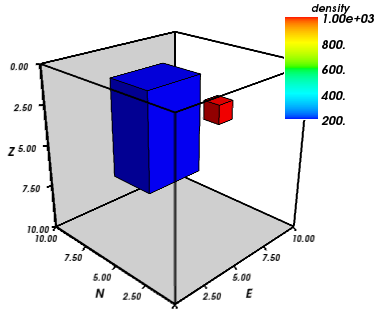
\includegraphics[width=0.7\textwidth]{figures/paper-fatiando/meshes_3dplotting_2prisms}
    \caption{
        Example of plotting a list of right rectangular prisms in Mayavi.
    }
    \label{fig:p1-twoprisms}
\end{figure}

The \texttt{fatiando.mesher} module also contains classes for
collections of elements (e.g., meshes). A good example is the
\texttt{PrismMesh} class that represents a structured mesh of right
rectangular prisms. This class behaves as a list of
\texttt{fatiando.mesher.Prism} objects and can be passed to functions
that ask for a list of prisms, like \texttt{fatiando.vis.myv.prisms}.
Physical properties can be assigned to the mesh using the
\texttt{addprop} method (Figure~\ref{fig:p1-mesh}):

\begin{verbatim}
mesh = mesher.PrismMesh(bounds, shape=(3, 3, 3))
mesh.addprop('density', range(mesh.size))
myv.figure()
myv.prisms(mesh, 'density')
myv.axes(myv.outline(bounds))
myv.show()
\end{verbatim}

\begin{figure}
    \centering
    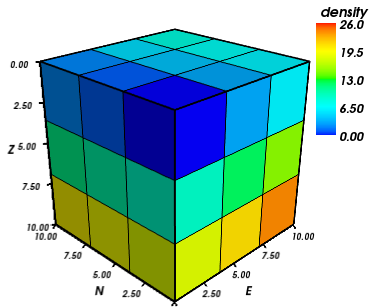
\includegraphics[width=0.7\textwidth]{figures/paper-fatiando/meshes_3dplotting_mesh}
    \caption{
        Example of generating and visualizing a structured prism mesh.
    }
    \label{fig:p1-mesh}
\end{figure}

Often times the mesh is used to make a detailed model of an irregular
region of the Earth's surface. In such cases, it is necessary to
consider the topography of the region. The \texttt{PrismMesh} class has
a \texttt{carvetopo} method that masks the prisms that fall above the
topography. The example below illustrates this functionality using
synthetic topography (Figure~\ref{fig:p1-meshtopo}):

\begin{verbatim}
from fatiando import utils
x, y = gridder.regular(bounds[:4], (50, 50))
heights = -5 + 5*utils.gaussian2d(x, y, 10, 5,
    x0=10, y0=10)
mesh = mesher.PrismMesh(bounds, (20, 20, 20))
mesh.addprop('density', range(mesh.size))
mesh.carvetopo(x, y, heights)
myv.figure()
myv.prisms(mesh, 'density')
myv.axes(myv.outline(bounds))
myv.wall_north(bounds)
myv.show()
\end{verbatim}

\begin{figure}
    \centering
    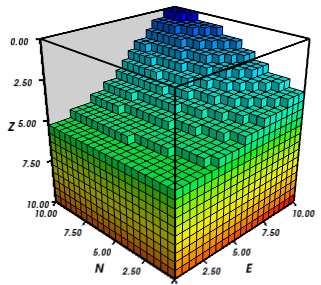
\includegraphics[width=0.7\textwidth]{figures/paper-fatiando/meshes_3dplotting_meshtopo}
    \caption{
        Example of generating and visualizing a prism mesh with masked
        topography.
    }
    \label{fig:p1-meshtopo}
\end{figure}

When modeling involves the whole Earth, or a large area of it, the
geophysicist needs to take into account the Earth's curvature. In such
cases, rectangular prisms are inadequate for modeling and tesseroids
(e.g., spherical prisms) are better suited. The
\texttt{fatiando.vis.myv} module contains auxiliary functions to plot
along with tesseroids: an Earth-sized sphere, meridians and parallels,
as well as continental borders (Figure~\ref{fig:p1-tesseroid}):

\begin{verbatim}
model = [
    mesher.Tesseroid(-60, -55, -30, -27, 500000, 0,
        props={'density':200}),
    mesher.Tesseroid(-66, -55, -20, -10, 300000, 0,
        props={'density':-100})]
fig = myv.figure(zdown=False)
myv.tesseroids(model, 'density')
myv.continents(linewidth=2)
myv.earth(opacity=1)
myv.meridians(range(0, 360, 45), opacity=0.2)
myv.parallels(range(-90, 90, 45), opacity=0.2)
# Rotate the camera to get a good view
scene = fig.scene
scene.camera.position = [21199620.406122234,
    -12390254.839673528, -14693312.866768979]
scene.camera.focal_point = [-535799.97230670298,
    -774902.33205294283, 826712.82283183688]
scene.camera.view_angle = 19.199999999999996
scene.camera.view_up = [0.33256519487680014,
    -0.47008782429014295, 0.81756824095039038]
scene.camera.clipping_range = [7009580.0037488714,
    55829873.658824757]
scene.camera.compute_view_plane_normal()
scene.render()
myv.show()
\end{verbatim}

\begin{figure}
    \centering
    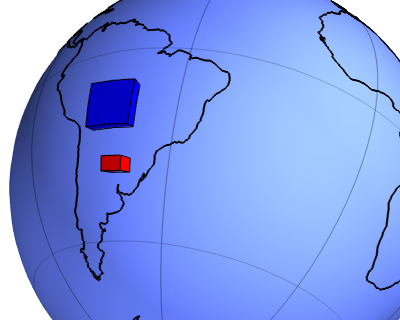
\includegraphics[width=0.7\textwidth]{figures/paper-fatiando/meshes_3dplotting_tesseroid}
    \caption{
        Example of creating a tesseroid (spherical prism) model and visualizing
        it in Mayavi.
    }
    \label{fig:p1-tesseroid}
\end{figure}




\section{Forward modeling}

In geophysics, the term ``forward modeling'' is used to describe the
process of generating synthetic data from a given Earth model.
Conversely, geophysical inversion is the process of estimating Earth
model parameters from observed data.

The Fatiando a Terra packages have separate modules for forward modeling
and inversion algorithms. The forward modeling functions usually take as
arguments geometric elements from \texttt{fatiando.mesher} with assigned
physical properties and return the synthetic data. For example, the
module \texttt{fatiando.gravmag.tesseroid} is a Python implementation of
the program Tesseroids (\url{http://leouieda.github.io/tesseroids}) and
calculates the gravitational fields of tesseroids (e.g., spherical
prisms). The following example shows how to calculate the gravity
anomaly of the tesseroid model generated in the previous section
(Figure~\ref{fig:p1-tesseroidgrav}):

\begin{verbatim}
from fatiando import gravmag
area = [-80, -30, -40, 10]
shape = (50, 50)
lons, lats, heights = gridder.regular(area, shape,
    z=2500000)
gz = gravmag.tesseroid.gz(lons, lats, heights, model)
mpl.figure()
bm = mpl.basemap(area, 'ortho')
bm.drawcoastlines()
bm.drawmapboundary()
bm.bluemarble()
mpl.title('Gravity anomaly (mGal)')
mpl.contourf(lons, lats, gz, shape, 30, basemap=bm)
mpl.colorbar()
mpl.show()
\end{verbatim}

\begin{figure}
    \centering
    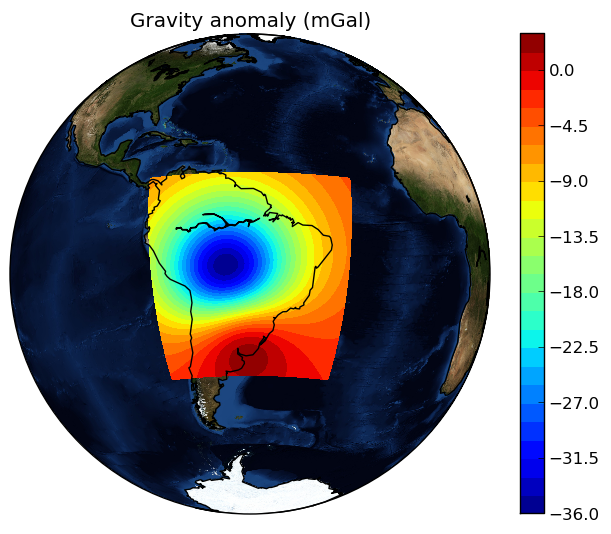
\includegraphics[width=0.7\textwidth]{figures/paper-fatiando/gravmag_tesseroid_data}
    \caption{
        Example of forward modeling the gravity anomaly using the tesseroid
        model shown in Figure~\ref{fig:p1-tesseroid}.
    }
    \label{fig:p1-tesseroidgrav}
\end{figure}

The module \texttt{fatiando.gravmag.polyprism} implements the method of
\citet{plouff1976} to forward model the gravity fields of a 3D right polygonal
prism. The following code sample shows how to interactively generate a
polygonal prism model and calculate its gravity anomaly
(Figures~\ref{fig:p1-drawing} and \ref{fig:p1-polyprism}):

\begin{verbatim}
# Draw a polygon and make a polygonal prism
bounds = [-1000, 1000, -1000, 1000, 0, 1000]
area = bounds[:4]
mpl.figure()
mpl.axis('scaled')
vertices = mpl.draw_polygon(area, mpl.gca(),
    xy2ne=True)
model = [mesher.PolygonalPrism(vertices, z1=0,
    z2=500, props={'density':500})]
# Calculate the gravity anomaly
shape = (100, 100)
x, y, z = gridder.scatter(area, 300, z=-1)
gz = gravmag.polyprism.gz(x, y, z, model)
mpl.figure()
mpl.axis('scaled')
mpl.title("Gravity anomaly (mGal)")
mpl.contourf(y, x, gz, shape=(50, 50),
    levels=30, interp=True)
mpl.colorbar()
mpl.polygon(model[0], '.-k', xy2ne=True)
mpl.set_area(area)
mpl.m2km()
mpl.show()
myv.figure()
myv.polyprisms(model, 'density')
myv.axes(myv.outline(bounds),
        ranges=[i*0.001 for i in bounds])
myv.wall_north(bounds)
myv.wall_bottom(bounds)
myv.show()
\end{verbatim}

\begin{figure}
    \centering
    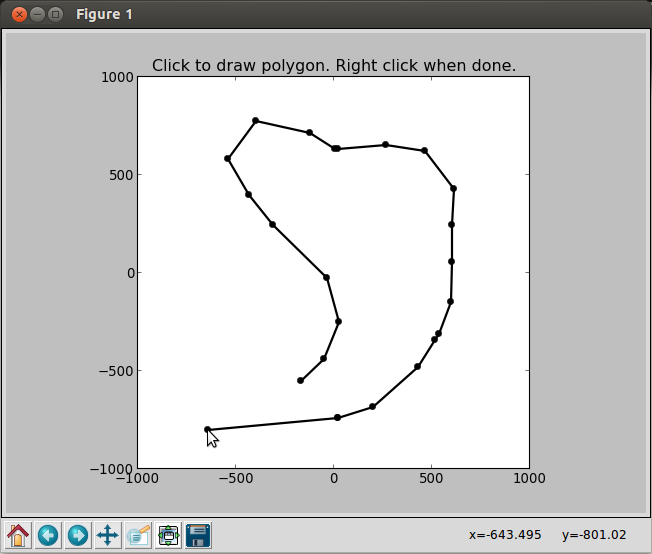
\includegraphics[width=0.7\textwidth]{figures/paper-fatiando/forward_modeling_polyprism_drawing}
    \caption{
        Screen-shot of interactively drawing the contour of a 3D polygonal
        prism, as viewed from above.
    }
    \label{fig:p1-drawing}
\end{figure}

\begin{figure}
    \centering
    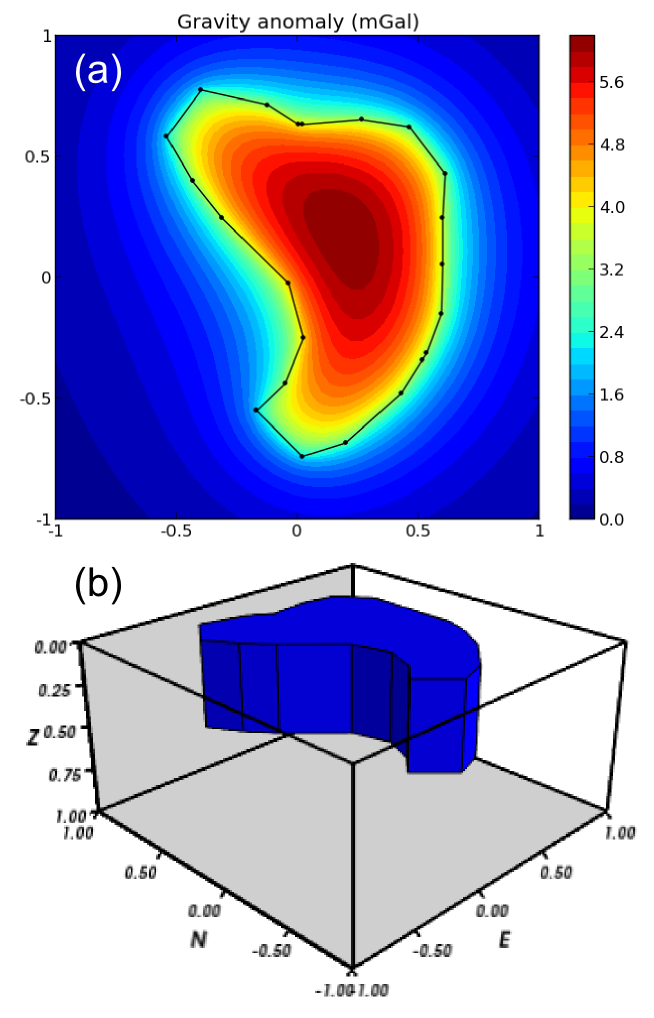
\includegraphics[width=0.5\textwidth]{figures/paper-fatiando/forward_modeling_polyprism}
    \caption{
        Example of forward modeling the gravity anomaly of a 3D polygonal
        prism.
        a) forward modeled gravity anomaly.
        b) 3D plot of the polygonal prism.
    }
    \label{fig:p1-polyprism}
\end{figure}




\section{Gravity and magnetic methods}

Geophysics uses anomalies in the gravitational and magnetic fields
generated by density and magnetization contrasts within the Earth to
investigate the inner Earth structure. The Fatiando a Terra 0.1 release
has been focused on gravity and magnetic methods. Therefore, the
\texttt{fatiando.gravmag} package contains more advanced and
state-of-the-art algorithms than the other packages.

The module \texttt{fatiando.gravmag.imaging} implements the imaging methods
described in \citet{fedi2012}. These methods aim to produce an image of the
geologic source from the observed gravity or magnetic data. The following code
sample uses the ``sandwich model'' method \citep{pedersen1991} to image the
polygonal prism, produced in the previous section, based on its gravity anomaly
(Figure~\ref{fig:p1-imaging}):

\begin{verbatim}
estimate = gravmag.imaging.sandwich(x, y, z, gz,
    shape, zmin=0, zmax=1000, nlayers=20, power=0.2)
body = mesher.vfilter(1.3*10**8, 1.7*10**8,
    'density', estimate)
myv.figure()
myv.prisms(body, 'density', edges=False)
p = myv.polyprisms(model, 'density',
    style='wireframe', linewidth=4)
p.actor.mapper.scalar_visibility = False
p.actor.property.color = (0, 0, 0)
myv.axes(myv.outline(bounds),
    ranges=[i*0.001 for i in bounds])
myv.wall_north(bounds)
myv.wall_bottom(bounds)
myv.show()
\end{verbatim}

\begin{figure}
    \centering
    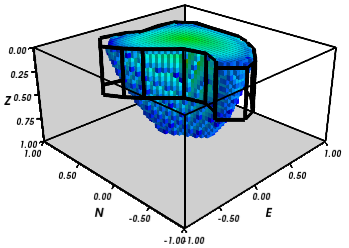
\includegraphics[width=0.7\textwidth]{figures/paper-fatiando/gravmag_imaging}
    \caption{
        Example of using the "sandwich model" imaging method to recover a 3D
        image of a geologic body based on its gravity anomaly. The colored
        blocks are a cutoff of the imaged body. The black contours are the true
        source of the gravity anomaly.
    }
    \label{fig:p1-imaging}
\end{figure}

Also implemented in Fatiando a Terra are some recent developments in
gravity and magnetic inversion methods. The method of ``planting
anomalous densities'' by \citet{uieda2012} is implemented in the
\texttt{fatiando.gravmag.harvester} module. In contrast to imaging
methods, this is an inversion method, i.e., it estimates a physical
property distribution (density in the case of gravity data) that fits
the observed data. This particular method requires the user to specify a
``seed'' (Figure~\ref{fig:p1-seed}) around which the estimated density
distribution grows (Figure~\ref{fig:p1-harvester}):

\begin{verbatim}
# Make a mesh and a seed
mesh = mesher.PrismMesh(bounds, (15, 30, 30))
seeds = gravmag.harvester.sow(
    [[200, 300, 100, {'density':500}]],
    mesh)
myv.figure()
myv.prisms([mesh[s.i] for s in seeds])
p = myv.polyprisms(model, 'density',
    style='wireframe', linewidth=4)
p.actor.mapper.scalar_visibility = False
p.actor.property.color = (0, 0, 0)
myv.axes(myv.outline(bounds),
    ranges=[i*0.001 for i in bounds])
myv.wall_north(bounds)
myv.wall_bottom(bounds)
myv.show()
# Now perform the inversion
data = [gravmag.harvester.Gz(x, y, z, gz)]
estimate = gravmag.harvester.harvest(data, seeds,
    mesh, compactness=0.1, threshold=0.0001)[0]
mesh.addprop('density', estimate['density'])
body = mesher.vremove(0, 'density', mesh)
myv.figure()
myv.prisms(body, 'density')
p = myv.polyprisms(model, 'density',
    style='wireframe', linewidth=4)
p.actor.mapper.scalar_visibility = False
p.actor.property.color = (0, 0, 0)
myv.axes(myv.outline(bounds),
    ranges=[i*0.001 for i in bounds])
myv.wall_north(bounds)
myv.wall_bottom(bounds)
myv.show()
\end{verbatim}

\begin{figure}
    \centering
    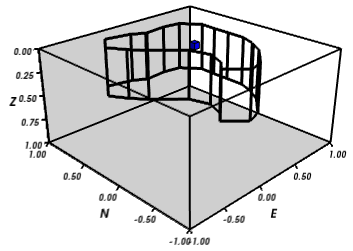
\includegraphics[width=0.7\textwidth]{figures/paper-fatiando/gravmag_harvester_seed}
    \caption{
        The small blue prism is the seed used by
        \texttt{fatiando.gravmag.harvester} to perform the inversion of a
        gravity anomaly. The black contours are the true source of the gravity
        anomaly.
    }
    \label{fig:p1-seed}
\end{figure}

\begin{figure}
    \centering
    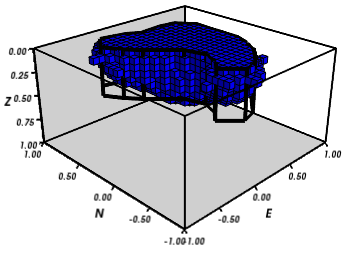
\includegraphics[width=0.7\textwidth]{figures/paper-fatiando/gravmag_harvester}
    \caption{
        The blue prisms are the result of a gravity inversion using module
        \texttt{fatiando.gravmag.harvester}. The black contours are the true
        source of the gravity anomaly. Notice how the inversion was able to
        recover the approximate geometry of the true source.
    }
    \label{fig:p1-harvester}
\end{figure}




\section{A toy seismic tomography}

The following example uses module \texttt{fatiando.seismic.srtomo} to
perform a simplified 2D tomography on synthetic seismic wave travel-time
data. To generate the travel-times we used a seismic wave velocity model
constructed from an image file. The colors of the image are converted to
gray-scale and the intensity is mapped to seismic wave velocity by the
\texttt{img2prop} method of the \texttt{fatiando.mesher.SquareMesh}
class. This model (Figure~\ref{fig:p1-tomo}) is then used to calculate the
travel-times between a random set of earthquake locations and seismic
receivers (seismometers):

\begin{verbatim}
import urllib
from fatiando import mesher, utils, seismic
from fatiando.vis import mpl
area = (0, 500000, 0, 500000)
shape = (30, 30)
model = mesher.SquareMesh(area, shape)
link = '/'.join(["http://fatiando.readthedocs.org",
    "en/Version0.1/_static/logo.png"])
urllib.urlretrieve(link, 'model.png')
model.img2prop('model.png', 4000, 10000, 'vp')
quake_locations = utils.random_points(area, 40)
receiver_locations = utils.circular_points(area, 20,
    random=True)
quakes, receivers = utils.connect_points(
    quake_locations, receiver_locations)
traveltimes = seismic.ttime2d.straight(model, 'vp',
    quakes, receivers)
noisy = utils.contaminate(traveltimes, 0.001,
    percent=True)
\end{verbatim}

Now the noise-corrupted synthetic travel-times can be used in our
simplified tomography:

\begin{verbatim}
mesh = mesher.SquareMesh(area, shape)
slowness, residuals = seismic.srtomo.run(noisy,
    quakes, receivers, mesh, smooth=10**6)
velocity = seismic.srtomo.slowness2vel(slowness)
mesh.addprop('vp', velocity)
# Make the plots
mpl.figure(figsize=(9, 7))
mpl.subplots_adjust(top=0.95, bottom=0.05,
    left=0.05, right=0.95)
mpl.subplot(2, 2, 1)
mpl.title('Velocity model (m/s)')
mpl.axis('scaled')
mpl.squaremesh(model, prop='vp', cmap=mpl.cm.seismic)
mpl.colorbar(pad=0.01)
mpl.points(quakes, '*y', label="Sources")
mpl.points(receivers, '^g', label="Receivers")
mpl.m2km()
mpl.subplot(2, 2, 2)
mpl.title('Ray paths')
mpl.axis('scaled')
mpl.squaremesh(model, prop='vp', cmap=mpl.cm.seismic)
mpl.colorbar(pad=0.01)
mpl.paths(quakes, receivers)
mpl.points(quakes, '*y', label="Sources")
mpl.points(receivers, '^g', label="Receivers")
mpl.m2km()
mpl.subplot(2, 2, 3)
mpl.title('Estimated velocity (m/s)')
mpl.axis('scaled')
mpl.squaremesh(mesh, prop='vp', cmap=mpl.cm.seismic,
    vmin=4000, vmax=10000)
mpl.colorbar(pad=0.01)
mpl.m2km()
mpl.subplot(2, 2, 4)
mpl.title('Residuals (s)')
mpl.hist(residuals, bins=10)
mpl.show()
\end{verbatim}

Even though the implementation in \texttt{fatiando.seismic.srtomo} is greatly
simplified and not usable in real tomography problems, the result in
Figure~\ref{fig:p1-tomo} illustrates interesting inverse problem concepts.  Notice
how the estimated velocity is blurred in the corners where no rays pass
through. This is because the data (travel-times) provide no information about
the velocity in those areas. Areas like those constitute the null space of the
inverse problem \citep{menke1984}, where any velocity value estimated will
provide an equal fit to the data.  Thus, the tomography problem requires the
use of prior information in the form of regularization. Most commonly used in
tomography problems is the Tikhonov first-order regularization, e.g., a
smoothness constraint \citep{menke1984}. The amount of smoothness imposed on
the solution is controlled by the \texttt{smooth} argument of function
\texttt{fatiando.seismic.srtomo.run}. That is how we are able to estimate a
unique and stable solution and why the result is specially smoothed where there
are no rays.



\begin{figure}
    \centering
    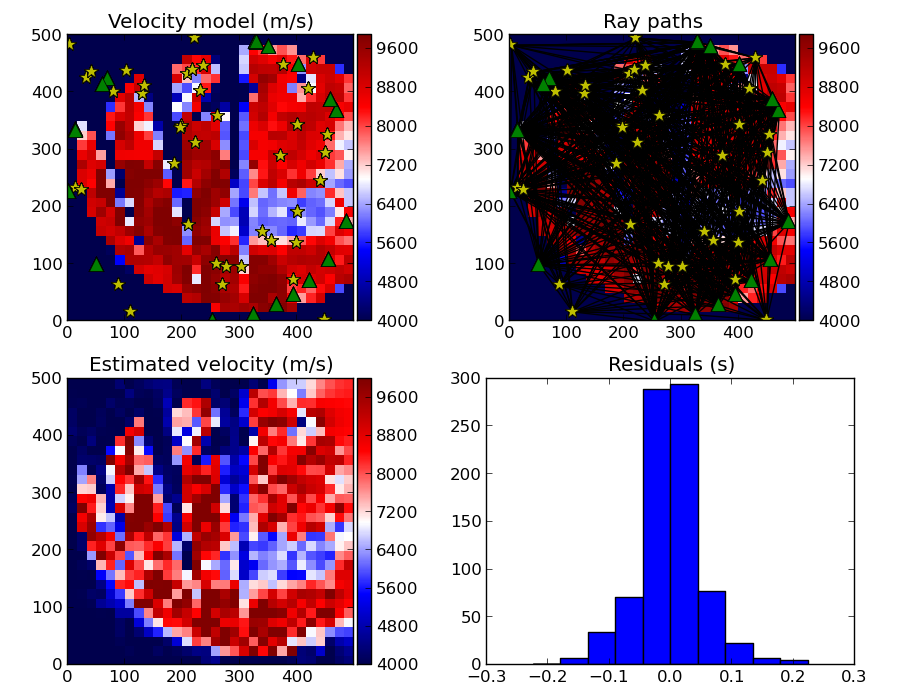
\includegraphics[width=\textwidth]{figures/paper-fatiando/seismic_tomo}
    \caption{
        Example run of a simplified 2D tomography. The top-left panel shows the
        true velocity model with the locations of earthquakes (yellow stars)
        and receivers (green triangles). The top-right panel shows the
        ray-paths between earthquakes and receivers. The bottom-left panel is
        the velocity estimated by the tomography. The bottom-right panel is a
        histogram of the travel-time residuals of the tomography. Notice how
        the majority of residuals are close to 0 s, indicating a good fit to
        the data.
    }
    \label{fig:p1-tomo}
\end{figure}




\section{Conclusion}

The Fatiando a Terra package provides an API to develop modeling
algorithms for a variety of geophysical methods. The current version
(0.1)\footnote{
    As of April 2016, the latest version is 0.3.}
has a few state-of-the-art gravity and magnetic modeling and
inversion algorithms. There are also toy problems in gravity, seismics
and seismology that are useful for teaching basic concepts of
geophysics, modeling, and inverse problems.

Fatiando a Terra enables quick prototyping of new algorithms because of
the collection of fast forward modeling routines and the simple syntax
and high level of the Python language. After prototyping, the
performance bottlenecks of these algorithms can be easily diagnosed
using the advanced profiling tools available in the Python language.
Optimization of only small components of code can be done without loss
of flexibility using the Cython language \citep{behnel2011}.

The biggest challenge that Fatiando a Terra faces in the near future is
the development of a user and, consequently, a developer community. This
is a key part for the survival of any open-source project.
